\documentclass[main.tex]{subfiles}

\begin{document}

\subsection{Secondo esercizio}

\begin{figure}[H]
\centering
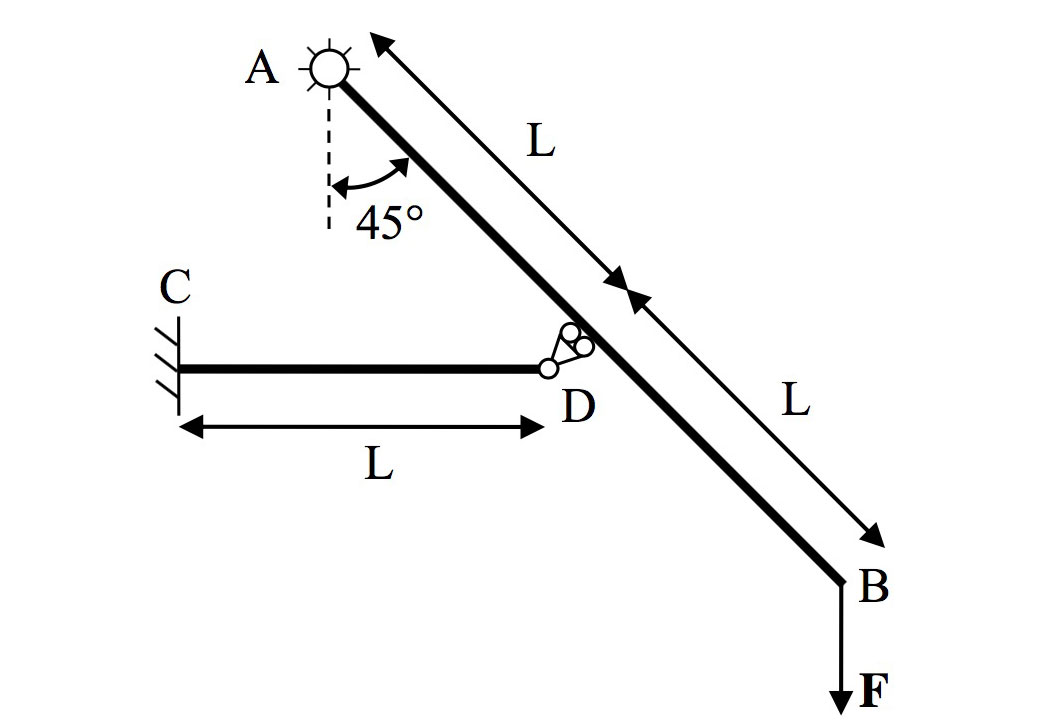
\includegraphics[width=0.75\textwidth]{2014-1009-2.jpg}
\end{figure}

La struttura in figura è soggetta al solo carico verticale F. Si chiede di calcolare:

\begin{enumerate}
\item Le reazioni vincolari in A e C.
\item Le azioni interne nell’asta AB (disegnare i corrispondenti diagrammi).
\end{enumerate}

\clearpage

\subsection{Soluzione secondo esercizio (non verificata)}

\subsubsection{Osservazioni}

\begin{enumerate}
\item La struttura è composta da 2 aste e 3 vincoli: un carrello, una cerniera esterna ed un incastro.
\item Il punto A \textbf{NON} si trova ad un'ascissa $x = \dfrac{L}{2}$ ma $x = L(1-\dfrac{\sqrt{2}}{2})$
\end{enumerate}

\subsubsection{Analisi preliminare di isostaticità}
Verifico che $gdl_{tot} = gdv_{tot}$:
\begin{figure}[H]
  \begin{subfigure}[b]{.5\textwidth}
  \centering
  \[
  	gdv: \begin{cases}
		gdv_{cerniera_{esterna}} = 2\\
		gdv_{incastro} = 3\\
		gdv_{carrello} = 1
  	\end{cases}
  \]
  \caption{Gradi di vincolo del sistema.}
  \end{subfigure}
  \hfill
  \begin{subfigure}[b]{.5\textwidth}
  \centering
  \[
  	gdl: \begin{cases}
  		gdl_{aste} = 6\\
  	\end{cases}  
  \]
  \caption{Gradi di libertà del sistema.}
  \end{subfigure}
  \caption{Verifica preliminare di isostaticità.}
\end{figure}

\subsubsection{Vincoli esterni}
Considerando il sistema come un corpo rigido, andiamo a sostituire le reazioni vincolari dei soli vincoli esterni (Figura \ref{vincoli_esterni_2014_1009_2}):

\[
	\begin{cases}
		H_A = -H_C \\
		V_A + V_C = F\\
		M_C + L\dfrac{\sqrt{2}}{2}H_A - L(1 - \dfrac{\sqrt{2}}{2})V_A + L(1+\dfrac{\sqrt{2}}{2})F = 0
	\end{cases}
\]

\begin{figure}[H]
\centering
\resizebox{.5\textwidth}{!}{% First image 2015 06 29

\begin{tikzpicture}

  \tiny


  \point{c}{0}{0}
  \point{c1}{0}{0.8}
  \point{c2}{-0.8}{0}
  \point{a}{2-1.41421}{1.41421}
  \point{a1}{2-1.41421}{0.8+1.41421}
  \point{d}{2}{0}
  \point{b}{2+1.41421}{-1.41421}
  \point{b1}{2+1.41421}{-1.41421-1.3}

  \beam{2}{c}{d}[0][1];
  \beam{2}{a}{b};

  \load{1}{a}[180][0.5]
  \load{1}{a1}[270][0.5]

  \load{2}{c}
  \load{1}{c}[180][0.5]
  \load{1}{c}[270][0.5]

  \load{1}{b1}[90][1]

  \notation{1}{c}{$\vec{M}_C$}[below right]
  \notation{1}{c}{$\vec{H}_C$}[below left]
  \notation{1}{c}{$\vec{V}_C$}[above right]

  \notation{1}{a}{$\vec{H}_A$}[below left]
  \notation{1}{a}{$\vec{V}_A$}[above right]

  \notation{1}{b}{$\vec{F}$}[below right]

  % \notation{1}{a1}{$\vec{H}_A$}
  % % \notation{1}{d1}{$\vec{R}_D$}
  % % \notation{1}{b1}{$\vec{H}_B$}[below left]
  % \notation{1}{c1}{$\vec{F}$}[above left]

  %  % \support{3}{o};

  %  % %Degrees
  %  % \notation{1}{o}{$\alpha$}[above];
  %  % \notation{1}{a}{$\beta$}[above];

  %  % \notation{5}{o}{a}[$a$];
  %  % \notation{5}{a}{b}[$b$];
  %  % \notation{5}{o}{b}[$c$];

\end{tikzpicture}}
\caption{Analisi dei vincoli esterni}
\label{vincoli_esterni_2014_1009_2}
\end{figure}

\subsubsection{Reazioni vincolari nell'asta CD}

\begin{figure}[H]
\centering
\resizebox{.5\textwidth}{!}{% First image 2015 06 29

\begin{tikzpicture}

  \tiny


  \point{a}{0}{0}
  \point{c}{1}{0}
  \point{b}{3}{0}
  \point{d}{1}{-1}


  \beam{2}{d}{c};

  \load{1}{d}[270][0.5]
  \load{2}{d}

  \load{1}{c}[0][0.5]
  \load{1}{c}[90][0.5]


  \notation{1}{d}{$\vec{M}_D$}[above]
  \notation{1}{d}{$\vec{H}_D$}[below left]
  \notation{1}{d}{$\vec{V}_D$}[below right]

  \notation{1}{c}{$\vec{V}_C$}[above right]
  \notation{1}{c}{$\vec{H}_C$}[below right]

\end{tikzpicture}}
\caption{Reazioni vincolari nell'asta CD}
\end{figure}

\[
	\begin{cases}
	R_{D_x} = H_C\\
	R_{D_y} = V_C\\
	M_C = -LR_{D_y} = -LV_C
	\end{cases}
\]

Siccome la rezione vincolare del carrello agisce ad un angolo di $45\deg$, è possibile affermare che: $R_{D_x} = R_{D_y}$.

Ne segue che:

\[
	\begin{cases}
	R_{D_x} = R_{D_y}\\
	H_C = V_C\\
	M_C = -LR_{D_y} = -LV_C
	\end{cases}
\]

Risolvo il sistema dei vincoli esterni sostituendo:

\[
	M_C = -LV_C;\quad
	V_A = F - V_C;\quad
	H_A = -H_C = -V_C;
\]

\begin{equation}
	M_C + L\dfrac{\sqrt{2}}{2}H_A - L(1 - \dfrac{\sqrt{2}}{2})V_A + L(1+\dfrac{\sqrt{2}}{2})F = 0
\end{equation}

\begin{equation}
	-LV_C - L\dfrac{\sqrt{2}}{2}V_C - L(1 - \dfrac{\sqrt{2}}{2})(F - V_C) + L(1+\dfrac{\sqrt{2}}{2})F = 0
\end{equation}

\begin{equation}
	-LV_C - L\dfrac{\sqrt{2}}{2}V_C  + L(1 - \dfrac{\sqrt{2}}{2})V_C - L(1 - \dfrac{\sqrt{2}}{2})F + L(1+\dfrac{\sqrt{2}}{2})F = 0
\end{equation}

\begin{equation}
	-\sqrt{2}V_C +\sqrt{2}F = 0
\end{equation}

\begin{equation}
	V_C = F
\end{equation}


\subsubsection{Ricapitolo soluzione primo punto}
\begin{figure}[H]
  \begin{subfigure}[b]{.5\textwidth}
  \centering
  \[
  	A: \begin{cases}
		H_A = -F\\
		V_A = 0
  	\end{cases}
  \]
  \caption{Reazioni vincolari in A.}
  \end{subfigure}
  \hfill
  \begin{subfigure}[b]{.5\textwidth}
  \centering
  \[
  	C: \begin{cases}
  		H_C = F\\
  		V_C = F\\
  		M_C = -LF
  	\end{cases}  
  \]
  \caption{Reazioni vincolari in C.}
  \end{subfigure}
\end{figure}

\subsubsection{Secondo punto}
Per meglio visualizzare le componenti di taglio e sforzo normale, ridisegno l'asta AB con i vettori secondo i versi corretti:

\begin{figure}[H]
\centering
\resizebox{.5\textwidth}{!}{% First image 2015 06 29

\begin{tikzpicture}

  \tiny


  \point{c}{0}{0}
  \point{c1}{0}{0.8}
  \point{c2}{-0.8}{0}
  \point{a}{2-1.41421}{1.41421}
  \point{a1}{2-1.41421}{0.8+1.41421}
  \point{d}{2}{0}
  \point{d1}{2-0.8}{0}
  \point{b}{2+1.41421}{-1.41421}
  \point{b1}{2+1.41421}{-1.41421-1.3}

  \beam{2}{a}{b};

  \load{1}{a}[0][1]
  % \load{1}{a1}[270][0.5]

  \load{1}{b1}[90][1]

  \load{1}{d}[180][1]
  \load{1}{d}[270][1]

  \notation{1}{a}{$\vec{H}_A$}[above right]

  \notation{1}{b}{$\vec{F}$}[below right]

  \notation{1}{d}{$\vec{R}_{D_x}$}[above left]
  \notation{1}{d}{$\vec{R}_{D_y}$}[below left]

  % \notation{1}{a1}{$\vec{H}_A$}
  % % \notation{1}{d1}{$\vec{R}_D$}
  % % \notation{1}{b1}{$\vec{H}_B$}[below left]
  % \notation{1}{c1}{$\vec{F}$}[above left]

  %  % \support{3}{o};

  %  % %Degrees
  %  % \notation{1}{o}{$\alpha$}[above];
  %  % \notation{1}{a}{$\beta$}[above];

  %  % \notation{5}{o}{a}[$a$];
  %  % \notation{5}{a}{b}[$b$];
  %  % \notation{5}{o}{b}[$c$];

\end{tikzpicture}}
\caption{Reazioni vincolari nell'asta AB con modulo e verso corretto}
\end{figure}

La forza $R_D$ impone solo un taglio, mentre le rimanenti impongono sia una componente di taglio che una di sforzo.

\[
R_D = \sqrt{2}F
\]

\paragraph{Sforzo normale}
Le forze $H_A$ ed $F$ impongono uno sforzo normale di \textbf{trazione}, quindi positivo.

\[
N = \dfrac{\sqrt{2}}{2}F
\]

\begin{figure}[H]
\centering
\resizebox{.5\textwidth}{!}{% First image 2015 06 29

\begin{tikzpicture}

  \tiny


  \point{c}{0}{0}
  \point{a}{0}{1}
  \point{b}{1}{0}
  \point{d}{2}{0}

   \beam{2}{c}{d}[0][1];

  \internalforces{c}{b}{1}{1}[0][blue];

\end{tikzpicture}}
\caption{Sforzo normale nell'asta AB}
\end{figure}

\paragraph{Taglio}
Le forze $H_A$ ed $R_D$ impongono una rotazione \textbf{anti-oraria}, quindi negativa, mentre le forze $R_D$ e $F$ una \textbf{oraria}, quindi, sempre seguendo la convenzione, positiva.

\[
T = \dfrac{\sqrt{2}}{2}F
\]

\begin{figure}[H]
\centering
\resizebox{.5\textwidth}{!}{% First image 2015 06 29

\begin{tikzpicture}

  \tiny


  \point{c}{0}{0}
  \point{c1}{0}{0.8}
  \point{c2}{-0.8}{0}
  \point{a}{2-1.41421}{1.41421}
  \point{a1}{2-1.41421}{0.8+1.41421}
  \point{d}{2}{0}
  \point{d1}{2-0.8}{0}
  \point{b}{2+1.41421}{-1.41421}
  \point{b1}{2+1.41421}{-1.41421-1.3}

  \beam{2}{a}{b};

  \internalforces{a}{d}{-0.707}{-0.707}[0][blue];
  \internalforces{d}{b}{0.707}{0.707}[0][red];

\end{tikzpicture}}
\caption{Taglio nell'asta AB}
\end{figure}

\paragraph{Momento flettente}
Il momento flettente raggiunge il valore massimo nel punto di taglio massimo, cioè D, in cui $M_{max} = \dfrac{\sqrt{2}}{2}LF$. Le fibre tese, in questo caso, si trovano sul lato di destra.

\begin{figure}[H]
\centering
\resizebox{.5\textwidth}{!}{% First image 2015 06 29

\begin{tikzpicture}

  \tiny


  \point{c}{0}{0}
  \point{c1}{0}{0.8}
  \point{c2}{-0.8}{0}
  \point{a}{2-1.41421}{1.41421}
  \point{a1}{2-1.41421}{0.8+1.41421}
  \point{d}{2}{0}
  \point{d1}{2-0.8}{0}
  \point{b}{2+1.41421}{-1.41421}
  \point{b1}{2+1.41421}{-1.41421-1.3}

  \beam{2}{a}{b};

  \internalforces{a}{d}{0}{-0.707}[0][red];
  \internalforces{d}{b}{-0.707}{0}[0][red];

\end{tikzpicture}}
\caption{Momento flettente nell'asta AB}
\end{figure}

\end{document}